\documentclass{article}
\usepackage{latexsym}
\usepackage[utf8]{inputenx}
\usepackage[spanish]{babel}
\usepackage{graphicx}
\usepackage{anysize}
\usepackage{amsmath}
\usepackage{amssymb}
\usepackage{float}
\setlength{\skip\footins}{5cm}
\usepackage{lscape}
\usepackage{verbatim}
\usepackage{moreverb}
\usepackage{url}
\usepackage{enumitem}
\usepackage{multicol}
\let\verbatiminput=\verbatimtabinput
\usepackage[nottoc,numbib]{tocbibind}
\setcounter{tocdepth}{4}
\setcounter{secnumdepth}{4}

\marginsize{2cm}{2cm}{.5cm}{3cm} 

\begin{document}

\begin{titlepage}

\newcommand{\HRule}{\rule{\linewidth}{0.5mm}} % Defines a new command for the horizontal lines, change thickness here

\center % Center everything on the page
 
%----------------------------------------------------------------------------------------
%	HEADING SECTIONS
%----------------------------------------------------------------------------------------

\textsc{\LARGE Universidad De Buenos Aires}\\[1.5cm] % Name of your university/college
\textsc{\Large Facultad De Ingeniería}\\[0.5cm] % Major heading such as course name
\textsc{\large 66.17 Sistemas digitales}\\[0.5cm] % Minor heading such as course title

%----------------------------------------------------------------------------------------
%	TITLE SECTION
%----------------------------------------------------------------------------------------

\HRule \\[0.4cm]
{ \huge \bfseries Voltímetro digital con salida VGA}\\[0.4cm] % Title of your document
\HRule \\[1.5cm]
 
%----------------------------------------------------------------------------------------
%	AUTHOR SECTION
%----------------------------------------------------------------------------------------

% If you don't want a supervisor, uncomment the two lines below and remove the section above
\Large Federico \textsc{Quevedo} - 93159\\ % Your name
[5cm] % Your name

%----------------------------------------------------------------------------------------
%	LOGO SECTION
%----------------------------------------------------------------------------------------


\includegraphics[scale=0.5]{UBA.jpg}\\[1cm] % Include a department/university logo - this will require the graphicx package

%----------------------------------------------------------------------------------------
%	DATE SECTION
%----------------------------------------------------------------------------------------

{\large \text \em {24 de Octubre de 2013}}\\[3cm] % Date, change the \today to a set date if you want to be precise
 
%----------------------------------------------------------------------------------------

\vfill % Fill the rest of the page with whitespace

\end{titlepage}

\tableofcontents
		
\newpage

\section{Objetivos}

El objetivo del presente Trabajo Práctico consiste en especificar, diseñar, describir una arquitectura, simular, sintetizar e implementar en FPGA un sistema digital para un voltímetro digital con salida VGA.

\begin{figure}[h!]
  \centering
	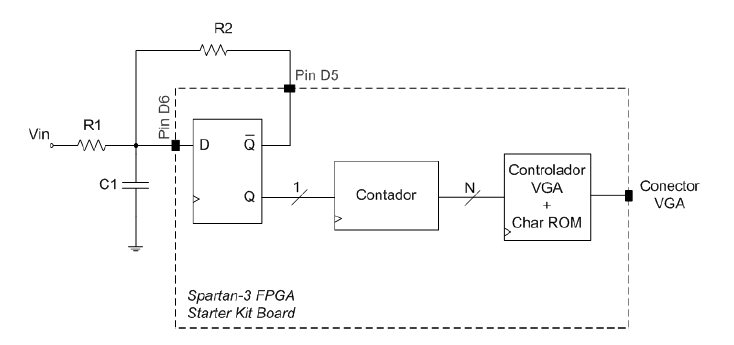
\includegraphics[scale=0.7]{diagramaEnBloques.png}\\[1cm] 
  \caption{Diagrama en bloques de la arquitectura propuesta.}
\end{figure}

\section{Modulos}

\subsection{Registro}

Se realizo una implementación simple de un registro usando un process que seteaba la salida a partir de las entradas.

\begin{verbatim}

entity registro is
     generic(N: integer:= 4);		-- valor genérico
     port(
          D: in std_logic_vector(N-1 downto 0);	-- entrada del registro
          clk: in std_logic;			-- señal de reloj
          rst: in std_logic;			-- señal de reset
          ena: in std_logic;		-- señal de habilitación
          Q: out std_logic_vector(N-1 downto 0)	-- salida del registro
     );
end;


architecture pp of registro is
begin
     process(clk, rst, ena)
     begin
          if rst = '1' then
               Q <= (others => '0');
          elsif clk = '1' and clk'event then
               if ena = '1' then
                    Q <= D;
               end if;
          end if;
     end process;
end;


\end{verbatim}


\subsection{Char ROM}

Para la memoria ROM se declaro un array de 255x8 donde se guarda la configuración de los números, ya que solo necesitamos los numeros del 0 al 9, el punto y la V, este array fue seteado en 0 desde la posicion 96 a la 255.

\subsection{Controlador VGA}

A través del controlador VGA ubicamos cada digito segun la fila y columna donde debia aparecer, obteniamos el digito correspondiente del contador de decadas y segun que numero era haciamos referencia a la dirección de la ROM donde se encontraba dicha representación.

\subsection{Conclusión}

Con la realización del presente trabajo se logro aprender a hacer una aplicación para FPGA con salida VGA, esto nos permite tener una representación grafica mucho más flexible que la limitada por hardward como pueden ser los leds o displays de 7 segmentos.

\end{document}